\documentclass[mscthesis]{usiinfthesis}
\usepackage{lipsum}
\usepackage{xcolor}
\usepackage{float}
\usepackage{cleveref}
\usepackage{makecell}
\usepackage{colortbl}
\usepackage{pdflscape}

\usepackage{listings}

\lstdefinelanguage{algebra}
{morekeywords={import,sort,constructors,observers,transformers,axioms,if,
else,end},
sensitive=false,
morecomment=[l]{//s},
}



\title{Design and implementation of a firewall system} %compulsory
\mastermajor{Financial Technology and Computing}%optional
\specialization{main track}
%\subtitle{Subtitle: Reinventing the World} %optional 
\author{Bin Yong} %compulsory
\begin{committee}
\advisor{Prof.}{Student's}{Advisor} %compulsory
\coadvisor{Prof.}{Student's}{Co-Advisor}{} %optional
\end{committee}
\Day{Yesterday} %compulsory
\Month{September} %compulsory
\Year{2023} %compulsory, put only the year
\place{Lugano} %compulsory

%\dedication{To my beloved} %optional
%\openepigraph{Someone said \dots}{Someone} %optional

%\makeindex %optional, also comment out \theindex at the end

\begin{document}

\definecolor{tablegray}{gray}{0.85}

\maketitle %generates the titlepage, this is FIXED

\frontmatter %generates the frontmatter, this is FIXED

\begin{abstract}
  \paragraph{}
  Design and implementation of a firewall system based on Raspberry Pi. The firewall will monitor and encrypt network activities. It is designed for someone who would like to sacrifice some compatibility to pursue better security but still wants some balance between security and convenience. A sensitive target, like an investigative journalist, could be a potential user of this device.

\end{abstract}

\begin{acknowledgements}
  \paragraph{}
  This document is a draft version of a working thesis of Bin Yong.
\end{acknowledgements}

\tableofcontents
\listoffigures %optional
\listoftables %optional

\mainmatter

\chapter{Introduction}
\paragraph{}
With the development of surveillance and management tools, people are losing controls of their own devices. Here are some facts that general publics may underestimated their impcats:

\begin{table}[H]
  \begin{enumerate}
    \item Any device with a microphone (sometimes a speaker may do the same) can know what sounds people are making around.
    \item Any device with a camera can 'see' what is happening around
    \item Any device connected to internet can upload what they know and receive commands from remote.
    \item Any device may have been hacked and functioning as not what they are designed.
    \item Some devices are designed with surveillance functionality.
  \end{enumerate}
  \caption{Some facts}
  \label{lst:facts}
\end{table}
Based on the facts above, some devices are naturally born with surveillance abilities. Take smartphones and smart speakers for example, they both hear voices and communicate with internet. Average people could not know what they actually uploaded to a remote server. They may only visually respond to "Hi, Siri." or "Hey, Alexa.", but they have to hear every sound happened around to achieve it. What if they keep uploading all of your conversations? Some are even worse: Intel Management Engine (Intel ME) or Intel Converged Security and
Management Engine (Intel CSME) and Intel Active Management Technology (Intel AMT) for example. It's obvious that they are made for management, a function that is unnecessray to most personal owners. According to their official documents. "its power stats are indpendent" means that simply powering off computer could not disable this management. "up before the main operating system" means that most users could not even notice it and can do nothing about it, and if something goes wrong, people cannot fix it by simply reinstalling operating system. It can access "LAN/Wireless LAN", check \cref{lst:facts}. "present on most Intel platforms, including client consumer and commercial systems, workstations, servers, and IoT (Internet of Things) products." means there is almost no escape. The details of its documents also shows the capability of running remote commands (Serial Over Local-Area Network), the capability of accessing local storage "Universial Serial Bus Redirect", "Keyboard, Video and Mouse" remote control over network.
\paragraph{}
So many things are out of control of the actual owners of the devices. People needs something to restrict the management and to show what is happening to the network. The goal of this work is to help on that. It is aimed to increase the chance of survival of the user from hacking, evasdropping, and digital fingerprinting. The device limits network activities and applies encryption standards to increase the difficulty of eavesdropping, and to reduce the attack surface of fingerprinting. It uses a screen to display selected real-time internet activities.
\paragraph{}
Using a hardware as a firewall has several advantages. Firstly, hardware
firewall is completely isolated between highly unsafe code,
like a browser, a video player, or a PDF reader. (fun fact: I was hacked repeatedly through personally harddened latest version of firefox while writing this thesis). This could also work as a mitigation of CPU/BIOS level threats: Firmware malwares, bootkits, and doubtable proprietray technologies like Intel ME and the AMD PSP. Second, it also provide convenience to the
user: the configuration of this portable device is applied to protect
everything behind it, so people do not need to do the time consuming
configuration work on different softwares and operating systems one by one.
\paragraph{}
Even things that could not be configured is under the restriction of the firewall. In example, people cannot untrust a built-in trusted root certificate from iPhone via Settings app.

\chapter{Hardware}
\section{Theory of the cost}
\paragraph{}
Commercial firewalls are usually more expensive than development boards that contains the same level of hardware functioality. One one hand, It's acceptable because they provided addtional values throught their software and services and all of the development and maintainance of the product, the service, and the company itself are costing money. On the other hand, it also indicates that an open-source solution like the tool introduced in this paper would reduce lower bound of the cost of accessing a hardware firewall.
\section{Market research on commercial firewalls}
\paragraph{}
Despite the firewall implemented in this paper is not a general purpose firewall, the difference in cost between market products is still worth knowing. From \cref{tab:amazon-search,tab:amazon-search-stat}, the prices of a firewall devices are around the price 250.74 EURO, and most of them are more expensive than the price of a Raspberry Pi 4B (68.79 EURO) selling on the same website. Only one exception: TP-LINK ER605. It's price is 55.5 euro which is still higher than the price of a Raspberry P 3B on the same website. After seeking into the details of this exception, its central management design and the corresponding cloud-based controller both showing that it is desigend for a totally different threat model and the its exceptional price could be explained, because it is under the control of that company and when people are motivated to spend money on a hardware firewall, their requirement to information security usually do not want to give full control of their firewall to a company. As a conclusion, using Raspberry Pi would cost less than usual general purpose firewalls.

\iffalse
  >>> x=[55.49,188.99,259.00,279.99,146.53,279.00,102.53,284.87,221.99,265.00,520.90,288.99,318.09,173.5,242.99,384.00]
  >>> sum(x)/len(x)
  250.74125000000004
  >>> import statistics
  >>> statistics.median(x)
  262.0
  >>> min(x)
  55.49
  >>> max(x)
  520.9
  >>> statistics.stdev(x)
  109.9844098573369
  >>> x=[188.99,259.00,279.99,146.53,279.00,102.53,284.87,221.99,265.00,288.99,318.09,173.5,242.99,384.00]
\fi
\begin{table}[H]
  \rowcolors{2}{tablegray}{}
  \begin{tabular}{|p{113mm}|p{12mm}|}
    \hline
    Name & Price   \\
    \hline
    \texttt{TP-LINK ER605 5 Port Dual/Multiple WAN VPN Router (up to 4 Gigabit WAN Ports, Highly Secure, Omada SDN, Central Management, Intelligent Monitoring, Firewall) Black, Ideal for Office Network
    }    & €55.49  \\
    \texttt{Micro Firewall Appliance, Mini PC, Pfsense Plus, Mikrotik, OPNsense, VPN, Router PC, Intel N4505, HUNSN RS41k, AES-NI, 4 x 2.5GbE I226-V, Console, Type-C, HDMI, DP, SIM Slot, 4G RAM, 32G SSD
    }    & €188.99 \\
    \texttt{ZyXEL ZyWALL 350Mbps VPN Firewall, Recommended for up to 10 Users [USG Flex 50]
    }    & €259.00 \\
    \texttt{Micro Firewall Appliance, Mini PC, pFsense Plus, Mikrotik, OPNsense, VPN, Router PC, Intel Alder Lake-N 12th Gen N100, HUNSN RJ42, 4 x 2.5GbE I226-V, 2 x HDMI, DP, TF, Type-C, 8G DDR5 RAM, 128G SSD
    }    & €279.99 \\
    \texttt{KingnovyPC Firewall Micro Appliance, 4 Port i226 2.5GbE LAN Fanless Mini PC N5100, 2* DDR4, HDMI, DP, RJ45 COM, 4*USB Gigabit Ethernet AES-NI VPN Router Openwrt Barebone
    }    & €146.53 \\
    \texttt{New J4125 Quad Core Firewall Micro Appliance, Mini PC, Nano PC, Router PC with 8G RAM 128G SSD, 4 RJ45 2.5GBE Port AES-NI Compatible with Pfsense OPNsense
    }    & €279.00 \\
    \texttt{Cisco Meraki Go - 5 Port Security Gateway - Power Supply to EU Standard GX20-HW-EU
    }    & €102.53 \\
    \texttt{Protectli Vault FW4B - 4 Port, Firewall Micro Appliance/Mini PC - Intel Quad Core, AES-NI, 4GB RAM, 32GB mSATA SSD - Compatible with pfSense/OPNsense etc
    }    & €284.87 \\
    \texttt{Firewall Hardware, Pfsense, OPNsense, Mikrotik, VPN, Network Security Appliance, Router PC, Intel Atom N2600, HHUNSN RS31, 4 x Intel Gigabit LAN, 2 x USB, COM, VGA, Fan, 4G RAM, 32G SSD
    }    & €221.99 \\
    \texttt{Firewall Mini PC with 2.5G Gigabit LAN, Firewall Micro Appliance Celeron J4125,4 x I225 Gigabit LAN,Fanless Mini PC AES-NI,12V,WiFi,HDMI,RS232 COM,USB 3.0,8GB RAM/128GB SSD
    }    & €265.00 \\
    \texttt{FORTINET FortiGate 40F Hardware - Next Generation Firewall Protection and Security
    }    & €520.90 \\
    \texttt{Micro Firewall Appliance, Mini PC, VPN, Router PC, Intel Alder Lake-N 12th Gen N100, HUNSN RJ42, 4 x 2.5GbE I226-V, 2 x HDMI, DP, TF, Type-C, Barebone, NO RAM, NO Storage, NO System
    }    & €288.99 \\
    \texttt{Cisco Systems Go Router Firewall Plus | Cloud Managed | VPN | Cisco [GX50-HW-EU], White
    }    & €318.09 \\
    \texttt{Zyxel Secure Cloud-Managed Router/Firewall with AXE5400 Tri-Band WiFi Subscription Free Network Security, Managed via Nebula APP/Ideal for Small Offices/Small Branches. [SCR 50AXE]
    }    & €173.5  \\
    \texttt{Micro Firewall Appliance, Mini PC, VPN, Router PC, Intel Alder Lake-N 12th Gen N100, HUNSN RJ46, 6 x 2.5GbE I226-V, 2 x HDMI2.1, TF, Type-C, Barebone, NO RAM, NO Storage, NO System
    }    & €242.99 \\
    \texttt{HSIPC 11th Gen i3 1115G4 Firewall Micro Appliance, Mini PC, Nano PC, Router PC (16G 256G) With 6 RJ45 2500M, AES-NI, HDMI USB3.0 Console, Compatible with Pfsense OPNsense
    }    & €384.00 \\
    \hline
  \end{tabular}
  \caption{The first page of search results of "hardware firewall" on amazon.de. Captured at 5 P.M. of December 26th, 2023, Lugano}
  \label{tab:amazon-search}
\end{table}

\begin{table}[H]
  \centering
  \begin{tabular}{|c|c|c|c|}
    \hline
    \multicolumn{4}{|c|}{Statistics of the prices in search results}                         \\
    \hline
    Mean                                     & 250.74                      & Median & 262.0  \\
    \hline
    Min                                      & 55.49                       & Max    & 520.89 \\
    \hline
    \multicolumn{2}{|c|}{Standard deviation} & \multicolumn{2}{c|}{109.98}                   \\
    \hline
  \end{tabular}
  \caption{Statistics of \cref{tab:amazon-search}}
  \label{tab:amazon-search-stat}
\end{table}

\section{Choosing Raspberry Pi}
\paragraph{}
The historical reason why Raspberry Pi is used is because it is the only single board computer (SBC) I have when this firewall started as a hobby project to solve the aggarsive hack problem that I was facing. The decision is unchanged after the start of this thesis mainly because the time costs on trying new SBCs: Since its first release on 2012, Raspberry Pi has upgraded its hardware models and software for multiple times, has accumluated a lot of working projects, and has maintained an active user community with a large number of experinced users behind it. All of them shows that using Raspberry Pi, I could cost less time on fixing the bugs of the SBC itself or on waiting for the answers from the community, because preivous users has asked and answered many questions and has found and fixed many problems. Besides that, its large number of users could also help on spreading the firewall project and help on pointing out security flaws of its new upgrades.

\chapter{Operating system}
\paragraph{}
Due to its security-focused nature, OpenBSD would be a great choice when buiding a firewall. However, as a portable device, it is designed to work as a USB network device but OpenBSD does not contain a device mode in its USB stack. Linux provides USB gadget mode. Using the combination of ECM and RNDIS mode, most of Linux, Windows, BSD and MacOS could be supported. FreeBSD USB stack can run in device mode and provided 3 virtual network iterface templates but none of them works with Microsoft Windows\citep{freebsdhb:usb}. Considering the large market share of Microsoft Windows, Linux is decided as the base OS of this firewall device.

\chapter{Packet filtering and forwarding}
\section{Design}
\paragraph{}
As the general principles, all traffics passed thorugh should be checked to against evasdropping. A plaintext connection should be channeled through strong encryptions or be discarded if unable to ensure its integrity.
\paragraph{}
A modern browser can satisify most of needs to interact with internet for working. So, allowing HTTP and HTTPS connections could make most of works done when facing a hostile network environment. Thus, everyting unnecessray to make this done are blocked. The firewall rules should be carefully made to filter out as much as possible and as early as possible, because everything on all layers of the Open Systems Interconnection model (OSI model) is protentialy vulnerable and the less network traffic being passed to the following components, the less chance a vulnerability can affect the firewall.
\paragraph{}
Proxies should be used to forward network traffics. There are advantages of using a proxy than forwarding packets like a router. First, a proxy can run under user level while packets forwarding run at kernel level. When there is a vulnerability, a userland one naturally to be less harmful than a kernel one. Second, proxies are easier and also safer to configure. It's hard to configure operatng system firewalls well. When the rules are not strict enough unexpected things may happen. In example, allowing any connection to 127.0.0.1 to success without a log, could cause potential problems if a malicious dhcp server assigned the address 127.0.0.1 to a physical network interface. Also, simply filtering packets by port numbers, addresses, and interfaces could not guarantee the packets being forwarded to the remote actually used by the protocols we are expecting. An attacker can simply let the receiving end of a reverse shell listen to an allowed port to bypass this kind of defense. By contrast, a proxy only works for the protocols that it can understand. when you are configuring a DNS proxy, the chance that your misconfiguration makes an attacker able to make http request over this proxy is very rare. They have to hack the firewall or create tunnels over those protocols to make their reverse shell work, which increased the difficulty of their operations. Third, the packets from the proxy are encoded again by Linux network stack so the fingerprinting techniques that targeting TCP ad IP properties is useless to the devices under its protection.

\section{Implementation}
\paragraph{}
Nftables is integrated in modern Linux systems. It can classify and filter network traffics. The firewall uses it to filter network packets. UDP 67 or 68 port and ARP packets are allowed for assigning IP addresses. UDP 53 is allowed from users to the firewall device for DNS requests, TCP 80, and TCP 443 are allowed for HTTP and HTTPS traffics. All other packets are filtered as early as possible.
\paragraph{}
Different proxies and RPC services are created to check connections, to forward traffcs, and to apply encryptions. Details are included in the chapters of the corresponding protocol. See \cref{fig:http-process-view,fig:ocsp-process-view,fig:tls-process-view}.

\chapter{Dynamic Host Configuration Protocol (DHCP)}

\section{Introduction}
\paragraph{}
DHCP is widely used to dynamically assign a ip address to a new device connected to a network.

\subsection{The issue}
\paragraph{}
A client can expose its host name to the network from the 'client identifier' option or 'sname' field in the protocol. When in the same local network, the host name exposed by the DHCP protocol and other protocols can be used to locate the devices of the victim. If the name of a computer is straightforward enough, like "Yongbin's MacBoook Pro", the network administrator will be able to know the name of the owner of the computer from the first glance. The hardware address exposed to the network can also expose more information than just the address. Hardware address or Media Access Control (MAC) address can be used to reversly lookup the manufacturer and the manufacturer can help identify the owner. In example, the network administrator may lookup the MAC address of the a device to find out the manufacturer is company A and if the company A only sell its products in Country B and if C is the only person come from Country B then the chance that the device belongs to C would be high.

\section{Design}
\paragraph{}
Firewall should randomize both host name and MAC address. The randomized computer name should look normal to prevent being identified by potential attackers.

\lstdefinelanguage{conf}{
basicstyle=\ttfamily\small,
columns=fullflexible,
morecomment=[s][\color{purple}\bfseries]{[}{]},
morecomment=[l]{\#},
commentstyle=\color{gray}\ttfamily,
morekeywords={},
otherkeywords={=},
keywordstyle={\color{green}\bfseries}
}

\section{Implementation}
\paragraph{}
NetworkManager is used to manage physical connections of the firewall. By adding 'ethernet.cloned-mac-address=random' and 'wifi.cloned-mac-address=random' to the 'connection' section of NetworkManager.conf, the MAC address randomization is done by NetworkManager. The 'ifconfig interface link random' command can also randomize the MAC address of a interface manually.
\paragraph{}
Host names of the firewall device is random generated while starting the system. The relevant code is inside rc.local. The name is crafted to look normal. The pattern of default computer name of Microsoft Windows and common names like iPad are used. Since the implementation of the client of the protocol could also be vulnerable, the combination of AppArmor and dhclient to mitigate this problem.
\paragraph{}
Dnsmasq is used to assign IP address of the users of the firewall it also tells the devices behind the firewall to use the firewall as the DNS resolver.

\chapter{Domain Name System (DNS)}

\section{Introduction}
DNS is a protocol that translates the human readable domain names to the ip addresses of the remote server. The default configuration of many devices are to use plaintexts to do requests, which could easily be monitored by simply recording the packets and be attacked by methods like DNS spoofing.

\section{Design}
\paragraph{}
From the network administrator's view, all DNS queries sent out from firewall shoul be encrypted. From the user's view, nothing should be specially configured.

\section{Implementation}
\subsection{Outgoing requests}
\paragraph{}
A name resoving service is created to resolve domain name queries from firewall serices. It is a local RPC service that resolve domain name queries via public DNS-over-HTTPS (DoH) services. DoH can mitigate both passive surveillance and DNS spoofing attacks\citep{rfc:doh8}. DoT (DNS-over-TLS) is another DNS encryption standard that can do almost the same as DoH. The reason why use DoH instead of DoT is that DoT uses a unique server port number, 853, that can be easily filtered and identified as an encrypted DNS connection, while DoH, with the help of using the same port number and protocol as HTTPS, makes it much harder to be identified and filtered than DoT.
\subsection{Inside firewall}
\paragraph{}
A dnsmasq is started locally to resolve everything to localhost to make the firewall proxy to be applied as system-wide.
\subsection{Incoming requests}
\paragraph{}
A dnsmasq is started to resolve everything to the firewall device to make the firewall proxy to be applied to devices behind it.

\chapter{Transport Layer Security (TLS)}

\section{Management of certificates}

\subsection{Introduction}
All modern major operating systems managed a collection of trused certificates issued by certificate authorities (CAs) they choose. Those certificates are used to prove the validity of a public key. When makeing a TLS connection, local applications check the path of the certificate provided by remote with local trusted collection to ensure secure connections.
\subsubsection{The issue}
\paragraph{}
Almost all TLS clients do not alert its user when the remote website presented a different certificate, which gives CAs the power to do man in the middle (MITM) attacks. Even if  do not want to do evil, their private key could still have been stolen. Thus, none of them are strictly trustworthy. However, whole TLS is based on it, if we trust none of those authorities, there will be almost no website we can use and if without TLS, things will only be worse.
\subsubsection{Exsting solutions}
\paragraph{}
SSL-pinning can prevent MITM attacks from a trusted CA when the user know the remote endpoint should use the certificate from another authority. However, configuring SSL-pinning to all the enspoints is hard and time consuming to average users and without a basic trusted environment, people unable to know whether the configuration has done correctly. Even if the configuration is correct, it is still not strange for an enspoint to switch to another CA. Thus, to a firewall, this technique cannot be used as a general solution of the issue that can be applied to all endpoints.
\paragraph{}
Removing suspecious CAs from the trusted list could protect people from MITM attacks initiated by those CA. However, some systems and devices do proide the function of untrusting a CA. In example, iPhone needs a computer to enable such configuration and most of Android variants.
\subsection{Design}
\paragraph{}
The firewall should trust only the CAs that are being widely used in the internet. People should be able to further decide which certificates to trust. One can consider untrust following when making such decisios: the CAs of the place you are staying, the CAs of the place you come from, and their enemies and allies.
\subsection{Implementation}
\paragraph{}
Since SSL-pinning can only be used on a small number of enspoints to an andvanced user who can clearly know what is this meant to be, it is not implemented now. Manually management of the certificate can be done by Linux commands. The certificate of all outgoing TLS connection remote points are checked by TLS proxy.

\section{Mismatch between the changing best current practice and the unchanged implementation}
\subsection{Problem}
The mismatch problem has been existed everywhere whenever a public protocol standard updated a fix to a problem. There are delays between a deficiency of a protocol being pubished and the majority of the implementation fixed the problem. A living example is that in the latest version of python 3.12.1 released on December 2023, as part of its builtin libraries, the implementation of the function create\_default\_context() from the ssl library is still creating a context that supports TLS 1.0 and TLS 1.1 by default \citep{pyton:ssl}, while they have already been deprecated by the best practice rfc8996 since March 2021 \citep{rfc:notls11}.

\subsection{Solution}
An idea to save the clients that contain severe deficiencies is to attack from their deficiencies then hijack and channel their communiction to remote endpoints through the TLS connection with the current best pracitces applied. The application of this methology to downgrade attack of Secure Socket Layer (SSL) version 2.0 was the initial motivation of the works on the TLS proxy, but the due to the drastic changes to the protocol, the final implementation is instead to use the proxy to check whether the best practice is applied.


\section{Proxy}
\subsubsection{MITM attack}
\paragraph{}
Despite using MITM attack to insepect or protect encrypted connections has been used in firewalls and proxies for many years \citep{fortigate:deepinspection}, the tls proxy used in this firewall should not implement the same functioality. The reason is that when the firewall itself is compromised, the ability to decrypt TLS sessions will cause a disasteer to the devices behind it: the attacker will be able to easily modify the encrypted data transfered over a MITM proxy while the devices behind the firewall will alert nothing about the modification. However, if the firewall could not do MITM attack at all, the compromised still unable to see and modify encryptions, because the certificate verification of the devices behind this firewall is still working.
\subsubsection{Filtering certificates}
\paragraph{}
The key\_share extension sometimes makes the certificate invisible to the proxy. Thus, in order to filter certificates, the proxy handshakes with remote server with a sepearate connection to verify the certificate used by the remote host. A cache of trusted endpoints is used to reduce delay caused by certificate check connections.

\subsubsection{Checking connections}
\paragraph{}
The proxy should parse handshake packets. It should check algorithms provided by ClientHello and ServerHello, to ensure strong encryption. Strenghten the connection by modifing handshake packets without MITM is not possible because the HMAC of all handshake packets is used for encryption.
\subsubsection{Implementation}

\begin{figure}[H]
  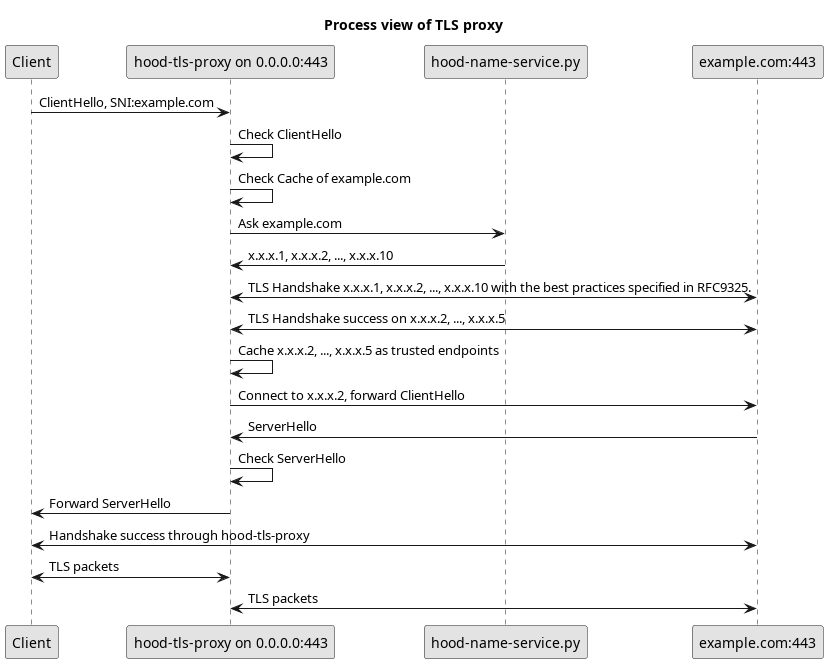
\includegraphics[width=\textwidth]{graphics/puml/process-tls-proxy.png}
  \caption{Process view of TLS proxy}
  \label{fig:tls-proxy-process-view}
\end{figure}

\paragraph{Programming language}
Since TLS proxy in charge of processing and forwarding the majority traffic of the firewall, c++ is used to develop the proxy due to its high performance capability.
\paragraph{ClientHello}
Upon receiving ClientHello from a client, the proxy at first check the version of the protocol, and the suppor\_versions extension to see if the client supports to establish a safe TLS channel, TLS 1.1 and TLS 1.2 are the only allowed versions \citep{rfc:bstprc}, if a ClientHello shows that the client supports neither, it will be discarded. After the version check, proxy checks ciphersuites field, if it contains none of the value listed in \ref{lst:tls-ciphersuites} \citep{rfc:bstprc}, it will be considered unable to be safe and discarded. If the ClientHello passed all of the security checks, the proxy will extract the Server Name Indication (SNI) from ClientHello to dertermine the actual destination of the request.

\begin{table}[H]
  \begin{itemize}
    \item TLS\_ECDHE\_RSA\_WITH\_AES\_128\_GCM\_SHA256
    \item TLS\_ECDHE\_RSA\_WITH\_AES\_256\_GCM\_SHA384
    \item TLS\_ECDHE\_ECDSA\_WITH\_AES\_128\_GCM\_SHA256
    \item TLS\_ECDHE\_ECDSA\_WITH\_AES\_256\_GCM\_SHA384
    \item TLS\_AES\_128\_GCM\_SHA256
    \item TLS\_AES\_256\_GCM\_SHA384
    \item TLS\_CHACHA20\_POLY1305\_SHA256
  \end{itemize}
  \caption{Allowed cipher suites values}
  \label{lst:tls-ciphersuites}
\end{table}

\paragraph{Name resolving and trused endpoint}
The proxy at first check if there is any cached trused endpoints available, if not it uses a RPC call to hood-name-service.py to resolve the domain name. Then TLS handshakes following the the same restrictions to the ClientHello check is made to all of the addresses returned from the name service. The handshake process will not only ensure remote endpoint meets the requirements (versions and ciphersuites) of applying the best practices described in rfc9325, it will also check whether the remote endpoint could provide a validate certificate of the hostname from a trusted CA of the firewall.
\paragraph{ServerHello} After forwarding the ClientHello to the server, a ServerHello will be responded and the proxy will check the final result of the handshake applies to the best practice. If a naughty attacker made the negotiation result to use unsafe, TLS 1.0 or the cipher suite RSA\_WITH\_NULL\_MD5 for example, the connection will be blocked.


\section{Process view of traffics}
\begin{figure}[H]
  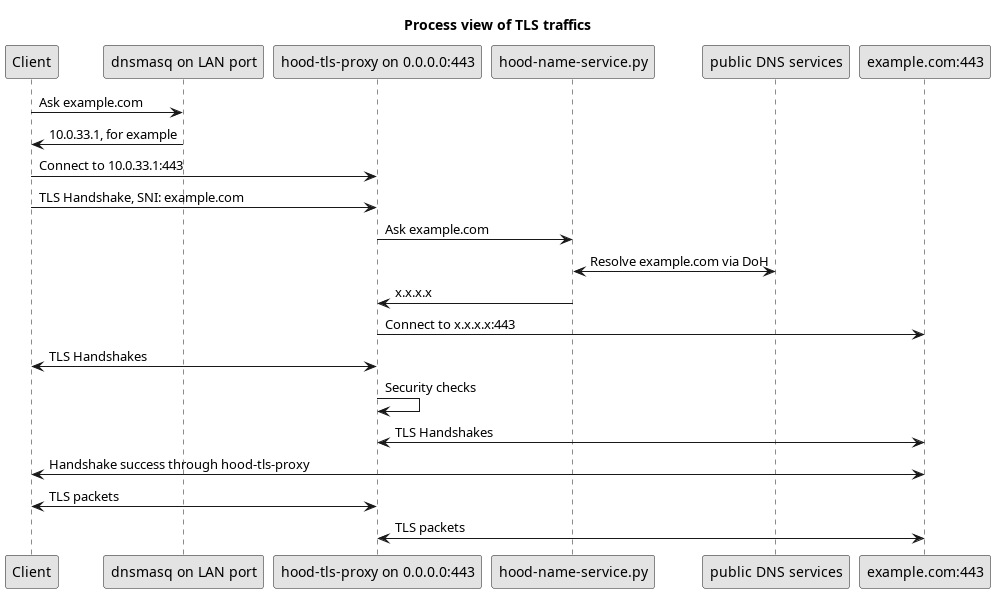
\includegraphics[width=\textheight, angle=90]{graphics/puml/process-tls-traffic.png}
  \caption{Process view of TLS traffics from user}
  \label{fig:tls-process-view}
\end{figure}

\chapter{Plaintext connections}

\section{HTTP}
\subsection{Implementation}
\paragraph{}
hood-http-handler.py is the proxy created to filter and protect HTTP plaintext connections. The proxy check the host name with a known list of OCSP (Online Certificate Status Protocol) and CRL (Certificate Revocatoin List) servers. Only the connections to those servers are allowed to be plaintext because those connections usually to be OCSP over HTTP connections, which have no reason to be protected. The connections to other servers are tunneled via TLS protocol through hood-tls-proxy service. See \cref{fig:ocsp-process-view,fig:http-process-view}.

\begin{figure}[H]
  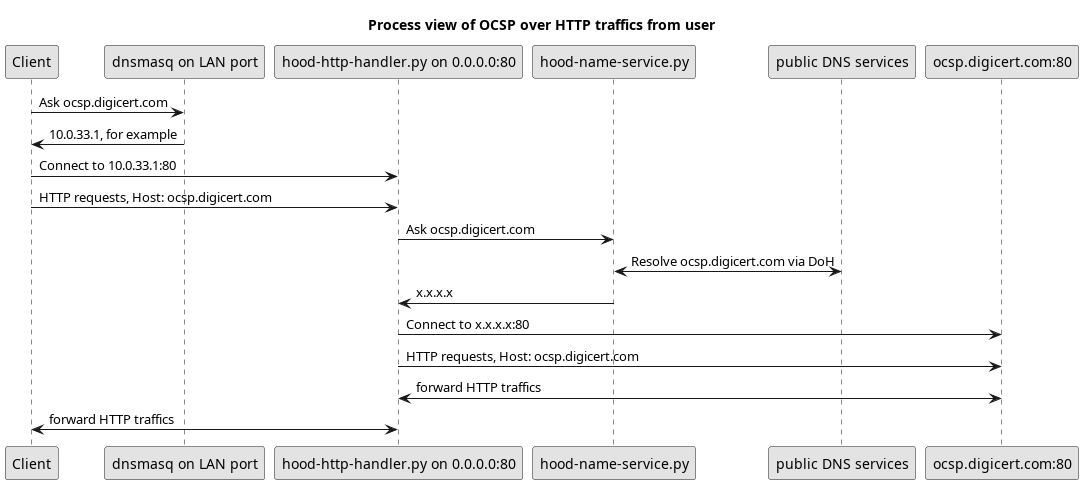
\includegraphics[width=\textheight, angle=90]{graphics/puml/process-ocsp-traffic.png}
  \caption{Process view of OCSP over HTTP traffics from user}
  \label{fig:ocsp-process-view}
\end{figure}

\begin{figure}[H]
  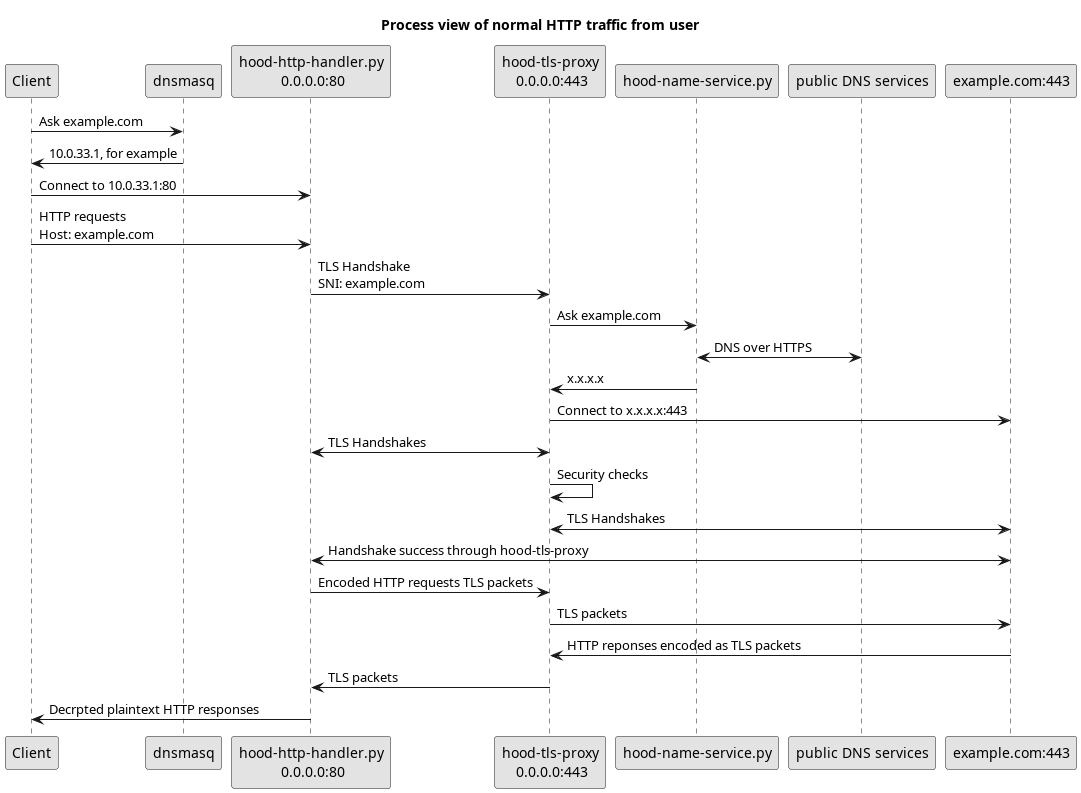
\includegraphics[width=\textheight, angle=90]{graphics/puml/process-http-traffic.png}
  \caption{Process view of normal HTTP traffics from user}
  \label{fig:http-process-view}
\end{figure}

\chapter{Date time synchornization}
\section{Introduction}
\paragraph{}
A correct time is required for TLS protocol to check certificates. Network Time Protocol (NTP) is used by most of modern systems to synchornize the clock with a remote server.
\subsection{The issue}
\paragraph{}
A problem of using a hardware like a Raspberry Pi is that it does not have a battery to keep the clock ticking after the power source is cut. So a time synchornization mechanism is a must for this firewall.
\paragraph{}
Many of operating systems are pre-configured to use a NTP server which having a unique domain name that can be used by a network administrator to identify the operating systems being used by the client.
\paragraph{}
Both the unique port number (UDP 123) and the unique domain names (time.windows.com, time.apple.com, and ubuntu.pool.ntp.org) makes NTP a protocol that can be easily identified and targeted. Various attacks can be done to the protocol itself\citep{ntp:attack}. The different in NTP behavior between different operating systems has been used in OS fingerprinting and tethering detection {osandtether}. Not to mention that the operating system being exposed by the domain name can also help an attacker to target the NTP client being used by the device.

\section{Design}
\paragraph{}
Give up on NTP, use HTTP/HTTPS instead. Use the "Date" header from the response of a HTTP server to synchornize date time in an acceptable accuracy. In order to hide from security detections, the attack vectors targeted to HTTP/HTTPS protocol usuall do not want to make mistakes in the header. Even if an attacker targeted to the method used by hood firewall, It's hard to say whether this request is made for time synchornization. Thus the date field of a HTTP response is generally trustworthy.

\section{Implementation}
\paragraph{}
The tool is implemented in a python script named hood-timesync.py. It accepts two command line arguments as listed in \cref{tab:timesync_cmdarg}. It at first try to receive a HTTP response through TLS connection from the domain name specified by host argument. If it failed, the reason could be the website is down or the system time is too different from the actual time and made a vailid certificate unable to pass the validation. Thus, a plaintext connection to the host name provided by the last resort address argument is made as the second attemept. After the second attempt, the tool starts another attempt to receive time from the domain of the host argument via TLS connection, because TLS has less chance to be attacked and because the reason why the first step failed could be the website is temporarily down, the reason could also be the huge time difference made the validation of the certificate failed. In both cases, a HTTPS request to the domain may become possible to success after the second attempt. An Epoch time is used as an 'achor' tim. Based on the assumption that time only moves forward, any time before this value will be rejected.

\begin{table}[H]
  \centering
  \begin{tabular}{|c|c|c|m{68mm}|}
    \hline
    Name               & Type & Default      & Description                                                                                                                                                                                                                                               \\
    \hline
    --host             & str  & www.bing.com & The website to request time from                                                                                                                                                                                                                          \\
    --last-resort-host & str  & 1.1.1.1      & The website used as the last resort, should be an IP address                                                                                                                                                                                              \\
    --time-anchor      & int  & 1703703361   & An Epoch time that being anchored as past.\newline Based on the assumption that time only moves forward, any time before this value will be rejected.\newline Set 0 to disable this test.\newline Example: -\-time-anchor=\$(stat /etc/os-release -c \%W) \\
    \hline
  \end{tabular}
  \caption{Command line arguments of hood-timesync.py}
  \label{tab:timesync_cmdarg}
\end{table}

\chapter{Behavioral simulation}
\section{Introduction}
\paragraph{}
In previous chapters, the fact that network activities can be used to detect the user has been proved in different protocols. However, the efforts to reduce the leak of the information on those protocols are not enought when facing a more sophisticated network analyzation. In example, the connections to Windows update servers and App Store servers can be used to detect Windows and Apple devices citep{osandtether}, but the firewall has no reason to stop those connections. Even if the firewall blocked all OS specific connections, the domain leaked from TLS handshakes can also tell the evasdroppers what websites a person is watching and then may infer what the person is doing. Thus, the leak of the information seems to be inevitable.

\section{Design}
\paragraph{}
A service to simuluate different network activities is designed to solve ths issue. The goal is to hide user network activities inside the flood of fake network activities to increase the difficulty of an analyzer to produce useful reports. However, the risk of using this service is to produce a false alarm immediately and make the user blocked for tethering, make the user fired for browsing unrelated websites, etc.. To avoid the firewall to be compromised from browser vulnerabilities, browser-based simulation tools, like puppeteer, should not be used for implementation. It should also make plaintext traffics to attaract attentions from attackers and evasdroppers to make them less focused on the actual user traffics.

\section{Implementation}
\paragraph{}
The service is implemented in a python script named hood-actor.py. It can parse and execute action files. To simuluate the behaviors of a human user or a computer service. All implementations inside script are based on the base modules of python, to avoid the version management of thrid party libraries being involved in the installation process of the firewall.

\subsection{Action files}
\paragraph{}
Action files are in JSON format. An action file contains an array of objects. All objects in the array has a "type" field to let the parser know how to process it. Supported object types are descripted in \cref{tab:action_type,tab:properties_object,tab:task_object}.

\begin{table}[H]
  \centering
  \begin{tabular}{|c|c|}
    \hline
    Value      & Description                    \\
    \hline
    properties & Properties of the action       \\
    task       & Tasks to be done in the action \\
    \hline
  \end{tabular}
  \caption{"type" field of action file objects}
  \label{tab:action_type}
\end{table}


\begin{table}[H]
  \centering
  \begin{tabular}{|c|c|c|}
    \hline
    Field       & Type                           & Description                     \\
    \hline
    type        & string                         & "properties"                    \\
    safe\_age   & integer                        & Minimum age safe to do this     \\
    proper\_age & list of two numbers [min, max] & Proper range of age to do this. \\
    \hline
  \end{tabular}
  \caption{"properties" object of action file}
  \label{tab:properties_object}
\end{table}

\begin{table}[H]
  \centering
  \begin{tabular}{|p{34mm}|p{26mm}|p{65mm}|}
    \hline
    Field                   & Type                           & Description                                          \\
    \hline
    type                    & string                         & "task"                                               \\
    name                    & string                         & Name of the task, must be unique in current file     \\
    before                  & list of strings                & Names of tasks that should run no earlier than this. \\
    after                   & list of strings                & Names of tasks that should run before this.          \\
    delay\_between\_actions & list of two numbers [min, max] & Range of seconds to wait between actions.            \\
    actions                 & list of strings                & list hood action script                              \\
    \hline
  \end{tabular}
  \caption{"task" object of action file}
  \label{tab:task_object}
\end{table}

\subsection{HoodExecutor}
HoodExecutor is a general purpose multi-thread task executor for python. It can run and schedule tasks that has dependency relationships and delay requirements in parallel. It has a thread pool of workers to execute tasks and a single thread for scheduling delayed tasks. It is requred to simulate the paralleled requests sent out from real world browsers if without third party HTTP client based on asyncio. It is also the cornerstone of fullfilling all the execution requirements of the tasks and actions in an action file.

\subsection{Browser}\label{sec:browser}
A fake browser is creted to simuluate network activities of browsing is a general purpose multi-thread task executor for python. It records the cookies specified in the HTTP response headers and sends them out like a real browser. It parses the HTML content of the webpage to extract the resources to be loaded and load them in parallel just like a real browser. It uses headers that used by real browsers and uses different headers on different resoures just like a real browser. Cookiesare stored in memory and used in the running session. However, Due to security concerns, and also to reduce the performance impacts caused by the actor, fake browser will neither render the webpage [CVE-2023-6707, CVE-2023-6351, CVE-2023-6869, CVE-2023-5170] nor evaluate scripts [CVE-2023-6702, CVE-2023-5997, CVE-2023-5728, CVE-2023-5723] used by the webpage.

\subsection{Hood action script}
\paragraph{}
Hood action script is a script to describe actions to be done to the actor. Each line of the script can be seen as three parts: namespaces, command, and argument. For example, \newline "hood:browser:goto:http://www.example.com". "hood:browser:" is to refer browser namespace from hood namespace, "goto" is a command inside browser namespace to tell intepreter to use browser to load a webpage. "http://www.example.com" is the parameter of the "goto" command. In this example, it represents the url of the webpage to be loaded.
\subsubsection{hood:browser:goto command}
\paragraph{}
Its usage is "hood:browser:goto URL". Its effect is to use a fake browser (See \cref{sec:browser}) to load a URL. When the special value "random\_link" is used as the argument, actor randomly picks a link from the webpage currently loaded in the browser to go to, but nothing will be done if current webpage contains not links.
\subsubsection{hood:loop command}
\paragraph{}
Its usage is "hood:loop:CONDITION:COMMAND". It is used to declare a loop. Multiple conditions can be declared in CONDITION part by syntax "key=value[,key=value]". Currently only two types of conditions are implemented: "exit\_chance" and "delay". "exit\_chance" describes the chance of the loop to be stopped. "exit\_chance=0.33" means the loop has 33% chance of termination at the beginning of each loop, "0" means it will never has an end. "1" means the loop will never be executed. "delay" describes the range of delay between each loop. "delay=0-2.5" means the delay between each loop is from 0 seconds to 2.5 seconds. A Just-In-Time compiler is implemented to convert the CONDITION field into python code. The COMMAND part is the hood action script to be executed in the loop.

\begin{figure}[H]
  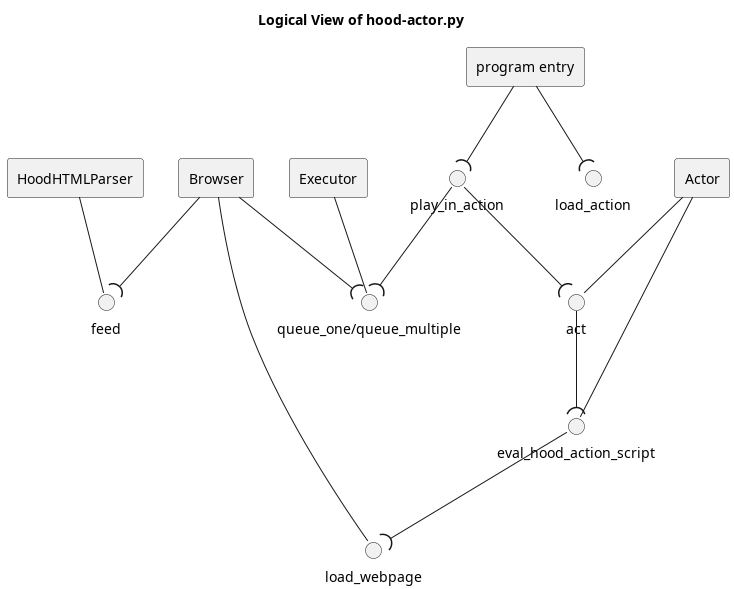
\includegraphics[width=0.9\textwidth]{graphics/puml/actor.png}
  \caption{Logic view of hood-actor.py}
  \label{fig:actor-logic-view}
\end{figure}

\chapter{Dispatcher and firewall rules}\label{cha:dispatcher}
\paragraph{}
Dispatcher is a shell script named 02-hood-dispatcher. It interacts with the changes of the network status or the system status to dynamically configure firewall rules and to start or stop netowrk services. It's callers are two sysrtemctl services: before-network.service (See \cref{sec:before-network-service}), udev.service, and NetworkManager-dispatcher.service.

\section{Initial state of firewall rules}
\paragraph{}
The initial state of firewall rules (See \cref{sec:nftables.conf}) is basic because the deisgn of nftables made the rules with interface name involved requires to be done dynamically. It only allows IPv4 and ARP protocol at layer 3. It allows anything to lo interface but reject anything else to communicate from 127.0.0.1 or to 127.0.0.1. It allows UDP/TCP packets in connection track established and related
state. It allows the device to send or receive ICMP fragmentation-needed packets. Anything else is ignored.

\section{On udev add event}
\subsubsection{netdev filter}
\paragraph{}
A default netdev filter will be added to both LAN and WAN interfaces. It has to be added dynamically because both of its ingress and egress filter requires the name of the device. The filter accepts only ARP and IP packets to passthrough. The firewall rules from other places already achieved the same thing but it is added because it is the earliest place to filter out a packet and the earlier a packet to be filtered the less chance the packet to cause a problem.

\section{On system startup}
\paragraph{}
Upon system startup, dispatcher will be called by before-network.service. It will start two dmesg instances one is for redirecting firewall related logs to a log file another is for formatting the log to a more human readable form. In iptables era, it was used for inititalizing iptables rules.
\paragraph{}
Since the udev event could be triggered at very early stage of the startup, so early that the nftables service may not available and adding rules may fail. Dispatcher try to add a netdev filter on all available network instances again because the timing before-network.service is sufficient to ensure the availability of nftables.service.

\section{On NetworkManager-dispatcher pre-up event}
\paragraph{}
This event means that a network interface is connected to the network but is not yet fully activated. The dispatcher checks the device path with the device specified during the installation process to know whether it is a WAN port. Devie path is the realpath of the network device. For example, on Linux, the device path of eth0 is the result of "realpath /sys/class/net/eth0".
\subsubsection{WAN port}
\paragraph{}
For the WAN port network interface, the dispatcher allows UDP packets to be sent out from local 68 port to remote 67 port and to be received from remote 67 port to local 68 port for DHCP protocol.
\subsubsection{LAN port}
\paragraph{}
For LAN port network interfaces, the dispatcher at first pick a randomized start number \(\in [2, 255]\) as the third byte of the IPv4 address, and all following LAN ports use the result of \[2 + (Last Used Number - 1) \mod 254\] as the third byte. The randomization of the start number is made after each system start. LAN subnet randomization could help increase the difficulty of a malicious code to detect the firewall from LAN port.
\paragraph{}
After randomization, following firewall rules is added:
\begin{table}[H]
  \begin{itemize}
    \item Accept the incoming TCP connections through the LAN interface if the destination IP address is the LAN IP address and the destination port is 80 or 443. For hood-http-handler.py and hood-tls-proxy
    \item Accept the incoming UDP packets through the LAN interface if the destination IP address is the LAN IP address and the destination port is 53. For the dnsmasq instance.
    \item Allow UDP packets to be sent out from local 67 port to remote 68 port and to be received from remote 68 port to local 68 port. For the dnsmasq instance.
  \end{itemize}
  \caption{Firewall rules to be added for LAN ports}
  \label{lst:LAN-rules}
\end{table}
\paragraph{}
A dnsmasq instance is started for this network interface, to assign IP addresses to connected devices, to let connected devices use the IP address of the LAN port of the firewall as the DNS server, and to respond the IP address of the LAN port for DNS requests.

\section{On NetworkManager-dispatcher up event}
Dispatcher only reacts to this event for the WAN port. It at first waits for DHCP to finish. After DHCP is done, dispatcher removes DHCP related accept rules from nftables and add a rule to accept outbound TCP connections from WAN instance with the source address as the DHCP result to remote 80 and 443 ports. This rule is for HTTP and HTTPS protocols. After that, dispatcher restarts the hood-network-services.service (\cref{sec:hood-network-services.service}). It will also check the existance of /do\_upgrade or /run\_once files to do system upgrade or to run the script.

\section{On NetworkManager-dispatcher down event}
Dispatcher removes the firewall rules dynamically added for this instance and kills the dnsmasq instances for this interface.

\chapter{Installation}
\paragraph{}
Installation now can only be done from Linux. install.sh is the shell script that in charge of the installation process. It copies and applies the scripts, executables, and configuration files to the target Raspberry Pi OS filesystem. It accepts the command line arguments listed in \cref{tab:install_arg}.

\begin{table}[H]
  \centering
  \begin{tabular}{|m{27mm}|m{30mm}|m{68mm}|}
    \hline
    Name                              & Default                                                                         & Description                                                                  \\
    \hline
    usb\_tether=                      & 1                                                                               & Share network to computer via USB cable                                      \\
    harden\_only=                     & 0                                                                               & Only apply hardening parts. Let the target SBC can still used as a computer. \\
    disable\_wireless=                & 1                                                                               & Disable WiFi and Bluetooth.                                                  \\
    disable\_gpu=                     & 1                                                                               & Disable GPU.                                                                 \\
    target=                           & /                                                                               & The target root/device to install firewall.                                  \\
    wan\_port\_\newline device\_path= & /sys/devices/\newline platform/scb/\newline fd580000.ethernet/\newline net/eth0 & The path of the device to be used as WAN port.                               \\
    \hline
  \end{tabular}
  \caption{Command line arguments of install.sh}
  \label{tab:install_arg}
\end{table}

\section{Checking target system}
Multiple checks to the target path are done before the beginning of the installation process to avoid potential harms to the user computer when they specified a wrong target path. It at first check the type of the target, if target path is not a directory target will be treated as a device or file and will be mounted as the pattern of a live system of Raspberry Pi OS. If target does not exist, "/dev/" prefix will be added and will be treated as a name of a device. Then if the content of /boot/firmware/config.txt of the target does not contain the string "dtparam", the target will not be treated as a Raspberry Pi OS filesystem and the installation process will be aborted.

\section{Disable wireless}
Multiple methods are used to ensure complete disable of wireless devices. See \cref{tab:config_disable_wireless,tab:delete_disable_wireless}.

\begin{table}[H]
  \centering
  \rowcolors{2}{tablegray}{}
  \begin{tabular}{|m{57mm}|m{68mm}|}
    \hline
    Configuration file                                    & Contents added                                                                                                                                                                                                     \\
    \hline
    boot/firmware/config.txt                              & dtoverlay=disable-bt\newline dtoverlay=disable-wifi                                                                                                                                                                \\
    /etc/modprobe.d/bin-y-disable-wireless-blacklist.conf & blacklist bluetooth\newline blacklist btbcm\newline blacklist hci\_uart\newline blacklist i2c\_brcmstb\newline blacklist i2c\_dev\newline blacklist brcmfmac\newline blacklist brcmutil\newline blacklist cfg80211 \\
    \hline
  \end{tabular}
  \caption{Configurations added to target to disable wireless}
  \label{tab:config_disable_wireless}
\end{table}

\begin{table}[H]
  \begin{itemize}
    \item /lib/firmware/brcm/*
    \item find /lib/linux-image*/broadcom -type f
    \item find /usr/lib/modules/ -name bluetooth
  \end{itemize}
  \caption{Files deleted from target to disable wireless}
  \label{tab:delete_disable_wireless}
\end{table}

\section{Disable GPU}
Multiple methods are used to ensure complete disable of GPU. See \cref{tab:config_disable_gpu,tab:delete_disable_gpu}.

\begin{table}[H]
  \centering
  \rowcolors{2}{tablegray}{}
  \begin{tabular}{|m{57mm}|m{68mm}|}
    \hline
    Configuration file                               & Contents modified                                                                                    \\
    \hline
    boot/firmware/config.txt                         & Removed:\newline dtoverlay=vc4-kms-v3d\newline dtoverlay=vc4-fkms-v3d                                \\
    /etc/modprobe.d/bin-y-disable-gpu-blacklist.conf & Added:\newline blacklist v3d\newline blacklist drm\newline blacklist drm\_panel\_orientation\_quirks \\
    \hline
  \end{tabular}
  \caption{Configurations modified to target to disable GPU}
  \label{tab:config_disable_gpu}
\end{table}

\begin{table}[H]
  \begin{itemize}
    \item Any directory under /usr/lib/modules/ with the name "gpu"
  \end{itemize}
  \caption{Files deleted from target to disable GPU}
  \label{tab:delete_disable_gpu}
\end{table}

\begin{landscape}
  \section{Other configurations modified}
  \begin{table}[H]
    \rowcolors{2}{tablegray}{}
    \begin{tabular}{|p{70mm}|p{40mm}|p{80mm}|}
      \hline
      Configuration file                                                                       & Contents modified                                                                                                   & Purpose                                                                            \\
      \hline
      /boot/firmware/cmdline.txt                                                               & Added:\newline ipv6.disable=1\newline apparmor=1\newline security=apparmor                                          & disable IPv6\newline enable AppArmor                                               \\
      /etc/modprobe.d/bin-y-blacklist.conf                                                     & Added:\newline blacklist ipv6\newline blacklist hci\_uart\newline blacklist i2c\_brcmstb\newline blacklist i2c\_dev & disable IPv6, i2c, and UART                                                        \\
      /boot/firmware/config.txt                                                                & Added:\newline enable\_uart=0                                                                                       & disable UART                                                                       \\
      /etc/nftables.conf                                                                       & See \cref{sec:nftables.conf}                                                                                        & nftables rules                                                                     \\
      /etc/hosts                                                                               & OMITTED                                                                                                             & provide addresss of some DNS services                                              \\
      /etc/sysctl.conf                                                                         & OMITTED                                                                                                             & sysctl related hardening                                                           \\
      /etc/rc.local                                                                            & OMITTED                                                                                                             & host name randomization                                                            \\
      /etc/pki/nssdb/cert9.db\newline /etc/pki/nssdb/key4.db\newline /etc/ca-certificates.conf & OMITTED                                                                                                             & manage trusted certificates                                                        \\
      /etc/NetworkManager/NetworkManager.conf                                                  & OMITTED                                                                                                             & MAC address randomization                                                          \\
      /etc/apt/sources.list\newline /etc/apt/sources.list.d/raspi.list                         & OMITTED                                                                                                             & use HTTPS mirrors for apt                                                          \\
      files related to systemd services                                                        & OMITTED                                                                                                             & enable hood services, enable required system services, and disable unsafe serivces \\
      \hline
    \end{tabular}
    \caption{Configurations modified to target to disable GPU}
    \label{tab:other_config}
  \end{table}
\end{landscape}

\chapter{Reasons of not to use}
\paragraph{}
In most cases, the reason to not use something is to reduce the attack surface.

\section{IPv6}
\section{WiFi}
\section{Bluetooth}
\section{GPU}
\section{Honeypot}

\chapter{Conclusions}

\section{Possible improvements for future}
\subsection{LSM and seccomp}
\paragraph{}
Use LSMs, like AppArmor, and seccomp to protect all as much process as possible. The programs that do not support seccomp can be changed by LD\_LOAD\_LIBRARY.

\subsection{Compile time hardening}
\paragraph{}
Use strict compiler options to harden everything, including kernel, like what Gentoo Linux is doing now, to try to mitigate some unpublished vulnerabilities, and also to increase the difficulty of attacking the firewall itself.

\subsection{Network stack fingerprinting}
\paragraph{}
Spoof network stacks, like TCP stacks and TLS stacks, to make the firewall and the devices behind it to be less detectable.

\subsection{Further use to libcomposite}
\paragraph{}
Libcomposite has the ability to make the device to show multiple roles to a host (a computer), which means the device can at the same time work as a USB mass storage device or as a USB CDROM, both of which can be used as a media of a Live DVD. Then the comptuer will be able to boot a live system from it. For a computer that password protected to boot from USB, we can also use this small device as a PXE server to make that computer boot from the network of the USB device.

\chapter{The attacks encountered during the time I was working on this thesis}

\section{Malicious hardwares}
\paragraph{}
Normal attackers will use network, bluetooth or wifi for communications between malware and the host. In example, casting the screen to another device via wifi or sending keyboard inputs via bluetooth. Those kind of attacks can be detected by a RF detector. RF sheilding fabrc, RF detectors, and signal jammers could be used to fight against such kind of attacks.
\paragraph{}
However, There are still other ways exist. Some even without wireless communications. Despite I have already bought a RF detector to alert me wireless communications between unknown hardwares, unknown attackers still managed to monitor my progress by modified hardwares. Take the devices that I am using to develop this project for example. Raspberry 4B has a usb chip that can communicate to the power source. If the charger is specially crafted with the ability to forward the usb connection to the remote endpoint via power lines, then, with the help from the malware installed on the pi itself, data can be leaked silently via power lines even without any network connections to the computer. The same story can also be happened to the portable screen that I am using now. I have found two counter measurements to this kind of attack: One is to use USB-C to DC adapter when connecting a USB-C charger to the laptop. Another is to tape the two pins in the middle of male USB-A port to prevent data communications.

\section{Sounds}

\paragraph{}
Another attack that can bypass a rfkilled computer is to use AI / ML to identify the sounds of keyboard hits. The detected types can be send to remote via power lines or mobile phones. The sound could even be recorded from the room of a neighbor which makes this attack more stealthy than other methods. I use cardboards to extend the pillar of the key cap to shorten the key travel to lower the volume of the sound of the key hit to counter this attack but I am uncertain about the effect because I have no attack tools to test this. AliPay also used to use sound waves to transmit data between phones and vending machines. My raspberry pi recently started to emit strange noises from the speakers on the screen, which could because of the same technology being used for hackers.

\appendix %optional, use only if you have an appendix

\chapter{Simple scripts and services created by firewall}

\section{before-network.service}\label{sec:before-network-service}
before-network.service is a systemd service being enabled during installation process and run before network is available to system. It is created to trigger dispatcher (See \cref{cha:dispatcher}) to initialize firewall rules and network configurations.

\section{hood-network-services.service}\label{sec:hood-network-services.service}
It is a service for running hood network services. It runs hood-network-services-runner.sh which starts hood-http-handler.py, hood-name-service.py, hood-tls-proxy, and a dnsmasq client for DNS queries made from the firewall system.

\section{nftables.conf}\label{sec:nftables.conf}
\begin{lstlisting}{language=conf}
#!/usr/sbin/nft -f

flush ruleset

table ip filter {
  chain input {
    type filter hook input priority filter; policy drop;
    iif lo accept
    ip daddr 127.0.0.1/8 log prefix "[HOOD D]" flags all drop 
    ip saddr 127.0.0.1/8 log prefix "[HOOD D]" flags all drop
    meta l4proto udp ct state {established, related} log prefix "[HOOD A]" flags all accept
    ct state {established, related} accept
    icmp type {destination-unreachable} icmp code {frag-needed} accept
    log prefix "[HOOD D]" flags all drop
  }
  chain forward {
    type filter hook forward priority filter; policy drop;
    log prefix "[HOOD D]" flags all drop
  }
  chain output {
    type filter hook output priority filter; policy drop;
    oif lo accept
    ip daddr 127.0.0.1/8 log prefix "[HOOD D]" flags all drop 
    ip saddr 127.0.0.1/8 log prefix "[HOOD D]" flags all drop 
    meta l4proto udp ct state {established, related} log prefix "[HOOD A]" flags all accept
    ct state {established, related} accept
    icmp type destination-unreachable icmp code {frag-needed} accept
    log prefix "[HOOD D]" flags all drop
  }
}

table ip6 filter {
  chain ingress {
    type filter hook input priority filter; policy drop;
    log prefix "[HOOD D]" flags all drop
  }
  chain prerouting {
    type filter hook input priority filter; policy drop;
    log prefix "[HOOD D]" flags all drop
  }
  chain input {
    type filter hook output priority filter; policy drop;
    log prefix "[HOOD D]" flags all drop
  }
  chain forward {
    type filter hook forward priority filter; policy drop;
    log prefix "[HOOD D]" flags all drop
  }
  chain output {
    type filter hook output priority filter; policy drop;
    log prefix "[HOOD D]" flags all drop
  }
  chain postrouting {
    type filter hook forward priority filter; policy drop;
    log prefix "[HOOD D]" flags all drop
  }
}

table bridge filter {
  chain ingress {
    type filter hook input priority filter; policy drop;
    log prefix "[HOOD D]" flags all drop
  }
  chain prerouting {
    type filter hook prerouting priority filter; policy drop;
    log prefix "[HOOD D]" flags all drop
  }
  chain input {
    type filter hook output priority filter; policy drop;
    log prefix "[HOOD D]" flags all drop
  }
  chain forward {
    type filter hook forward priority filter; policy drop;
    log prefix "[HOOD D]" flags all drop
  }
  chain output {
    type filter hook output priority filter; policy drop;
    log prefix "[HOOD D]" flags all drop
  }
  chain postrouting {
    type filter hook postrouting priority filter; policy drop;
    log prefix "[HOOD D]" flags all drop
  }
}

table netdev filter {
}


table arp filter {
  chain input {
    type filter hook input priority filter; policy drop;
  }
  chain output {
    type filter hook output priority filter; policy drop;
  }
}
\end{lstlisting}

\backmatter

\chapter{Glossary} %optional

%\bibliographystyle{alpha}
%\bibliographystyle{dcu}
\bibliographystyle{plainnat}
\bibliography{biblio}

%\cleardoublepage
%\theindex %optional, use only if you have an index, must use
%\makeindex in the preamble
%\lipsum
1
\end{document}
\grid
